%
% This is a borrowed LaTeX template file for lecture notes for CS267,
% Applications of Parallel Computing, UCBerkeley EECS Department.
% Now being used for CMU's 10725 Fall 2012 Optimization course
% taught by Geoff Gordon and Ryan Tibshirani.  When preparing 
% LaTeX notes for this class, please use this template.
%
% To familiarize yourself with this template, the body contains
% some examples of its use.  Look them over.  Then you can
% run LaTeX on this file.  After you have LaTeXed this file then
% you can look over the result either by printing it out with
% dvips or using xdvi. "pdflatex template.tex" should also work.
%
\documentclass[twoside]{article}
\usepackage{graphicx}
\usepackage{tikz}

\setlength{\oddsidemargin}{0.25 in}
\setlength{\evensidemargin}{-0.25 in}
\setlength{\topmargin}{-0.6 in}
\setlength{\textwidth}{6.5 in}
\setlength{\textheight}{8.5 in}
\setlength{\headsep}{0.75 in}
\setlength{\parindent}{0 in}
\setlength{\parskip}{0.1 in}
%
% ADD PACKAGES here:
%
\usepackage{amsmath,amsfonts,graphicx}
%
% The following commands set up the lecnum (lecture number)
% counter and make various numbering schemes work relative
% to the lecture number.
%
\newcounter{lecnum}
\renewcommand{\thepage}{\thelecnum-\arabic{page}}
\renewcommand{\thesection}{\thelecnum.\arabic{section}}
\renewcommand{\theequation}{\thelecnum.\arabic{equation}}
\renewcommand{\thefigure}{\thelecnum.\arabic{figure}}
\renewcommand{\thetable}{\thelecnum.\arabic{table}}
%
% The following macro is used to generate the header.
%
\newcommand{\lecture}[5]{
   \pagestyle{myheadings}
   \thispagestyle{plain}
   \newpage
   \setcounter{lecnum}{#1}
   \setcounter{page}{1}
   \noindent
   \begin{center}
   \framebox{
      \vbox{\vspace{2mm}
    \hbox to 6.28in { {\bf Physics 467/667: Thermodynamics/Statistical Physics
	\hfill Spring 2017} }
       \vspace{4mm}
       \hbox to 6.28in { {\Large \hfill Lecture #1: #2  \hfill} }
       \vspace{2mm}
       \hbox to 6.28in { {\it Lecturer: #3 \hfill Scribes: #4} }
      \vspace{2mm}}
   }
   \end{center}
   \markboth{Lecture #1: #2}{Lecture #1: #2}
   \vspace*{4mm}
}
%
% Convention for citations is authors' initials followed by the year.
% For example, to cite a paper by Leighton and Maggs you would type
% \cite{LM89}, and to cite a paper by Strassen you would type \cite{S69}.
% (To avoid bibliography problems, for now we redefine the \cite command.)
% Also commands that create a suitable format for the reference list.
\renewcommand{\cite}[1]{[#1]}
\def\beginrefs{\begin{list}%
        {[\arabic{equation}]}{\usecounter{equation}
         \setlength{\leftmargin}{2.0truecm}\setlength{\labelsep}{0.4truecm}%
         \setlength{\labelwidth}{1.6truecm}}}
\def\endrefs{\end{list}}
\def\bibentry#1{\item[\hbox{[#1]}]}
%Use this command for a figure; it puts a figure in wherever you want it.
%usage: \fig{NUMBER}{SPACE-IN-INCHES}{CAPTION}
\newcommand{\fig}[3]{
			\vspace{#2}
			\begin{center}
			Figure \thelecnum.#1:~#3
			\end{center}
	}
% Use these for theorems, lemmas, proofs, etc.
\newtheorem{theorem}{Theorem}[lecnum]
\newtheorem{lemma}[theorem]{Lemma}
\newtheorem{proposition}[theorem]{Proposition}
\newtheorem{claim}[theorem]{Claim}
\newtheorem{corollary}[theorem]{Corollary}
\newtheorem{definition}[theorem]{Definition}
\newenvironment{proof}{{\bf Proof:}}{\hfill\rule{2mm}{2mm}}
% **** IF YOU WANT TO DEFINE ADDITIONAL MACROS FOR YOURSELF, PUT THEM HERE:
\newcommand\E{\mathbb{E}}
\begin{document}
%FILL IN THE RIGHT INFO.
%\lecture{**LECTURE-NUMBER**}{**DATE**}{**LECTURER**}{**SCRIBE**}
\lecture{5}{The Second Law and Entropy}{Qiang Zhu}{scribe-name1,2,3}
%\footnotetext{These notes are partially based on those of Nigel Mansell.}
% **** YOUR NOTES GO HERE:
% Some general latex examples and examples making use of the
% macros follow.  
%**** IN GENERAL, BE BRIEF. LONG SCRIBE NOTES, NO MATTER HOW WELL WRITTEN,
%**** ARE NEVER READ BY ANYBODY.

\section{Some useful equations} % Don't be this informal in your notes!
\begin{equation} \label{idealgas} PV = nRT = NkT \end{equation}
\begin{equation} \label{Avogadro} N = n \times N_A \end{equation}
\begin{equation} \label{PV-micro} PV = Nm{\overline v_x^2} = NkT\end{equation}
\begin{equation} \label{eqpartition} U_{thermal} = N \cdot f \cdot \frac{1}{2}kT \end{equation}
\begin{equation} \label{1stlaw} \Delta{U} = Q + W \end{equation}
\begin{equation} \label{work3} \Delta W = - P \Delta{V} \end{equation}

\section{Introduction}

We have explored the law of energy conservation, and apply it to thermodynmic systems.
In the meantime, we studied the relations between heat, work and thermal energy,
and the connections between marcoscopic observables $P$, $V$, $T$ and miscroscopic properties $v$, $f$.

However, some very fundamental questions remain unanswered,
\begin{enumerate}
\item{\it what is temperature?}
\item{\it why does heat flow spontaneously from hot to cold object?}
\item{\it why does do many processes happen in one direction, but never the reverse?}
\end{enumerate}

\section{Combinatorics and Two-state systems}
Let's get started with a silly example of fliping three coins. How many possible outcomes are there?
\begin{tabular}{c c c}
Coin1 & Coin2 & Coin3 \\\hline
  H & H & H \\
  H & H & T \\
  H & T & H \\
  T & H & H \\
  H & T & T \\
  T & T & H \\
  T & H & T \\
  T & T & T \\\hline
\end{tabular}

In total we have 8 outcomes, each is called {\bf microstate}.\\
Since all coins are indistinguishable, we are more interested in how many heads are there in all outcomes?
By simply counting the number from the above table, we know \\
3 heads,  HHH 
2 heads,  HHT, HTH, THH \\
1 head,   HTT, TTH, THT \\
0 head,   TTT

each state is called {\bf microstate}.\\
{\bf microstate}: Each of the eight different outcomes\\
{\bf macrostate}: How many heads are there in all out comes\\

Although each microstate is equal to exist, but macrostates have different probabilies to explored.
Clearly, 2 heads is more likely to be found than 3 heads.
Here we introduce another quantity,\\
{\bf multiplicity ($\Omega$)}: the number of microstates in a given macrostate.\\

In the context of coin games, let's define $\Omega(n)$ as number of cases when we get $n$ heads.
If the total number of coins is $N$, we can derive the equations as follows,
\begin{equation}
 \Omega(N, n) = \frac{N!}{n!\cdot(N-n)!} = \binom{N}{n} 
\end{equation}

What will happen if we increase $N$. Let's try N = 4 and 20 in Problem 2.1 and 2.2.


Such two-state system is quite usual in physics, such as two-state paramagnet.

\section{The Einstein Model of a Solid}
$N$: Number of the osillators.\\
$q$: Number of energy states.

\begin{equation}
 \Omega(N, q) = \binom{q+N-1}{q} = \frac{(q+N-1)!}{q!(N-1)!}
\end{equation}

It can be simply proved as follows\\
$q$ circles; \\
$N-1$ vertical lines;\\
how to arrange them? \\
\begin{tikzpicture}
\draw (2,0) circle (0.2cm);
\draw (2.5,-0.5) -- (2.5,0.5);
\draw (3,0) circle (0.2cm);
\draw (4,0) circle (0.2cm);
\draw (4.5,-0.5) -- (4.5,0.5);
\draw (5,0) circle (0.2cm);
\draw (6,0) circle (0.2cm);
\draw (7,0) circle (0.2cm);
\end{tikzpicture}

{\bf Exercises}\\
Calculate the multiplicity of an Einstein solid with 5 oscillators and [1,2,3,4,5] units of Energy.\\
\begin{tabular}{c|c }
$q$ &$\Omega(5,q)$ \\\hline
 1     &  \\
 2     &  \\
 3     &  \\
 4     &  \\
 5     &  \\\hline
\end{tabular}

{\bf Computer programming}
\begin{enumerate}
\item Write a small piece of program to calculate $\Omega(N)$ in the context of flipping coins and plot them when $N$=10, 15, 30, 100.
\item Write a small piece of program to calculate $\Omega(N)$ in the context of Einstein solid and plot them when $N$=10, 15, 30, 100 and $q$ from 0 to 10.
\end{enumerate}

\begin{figure}[h]
\centering
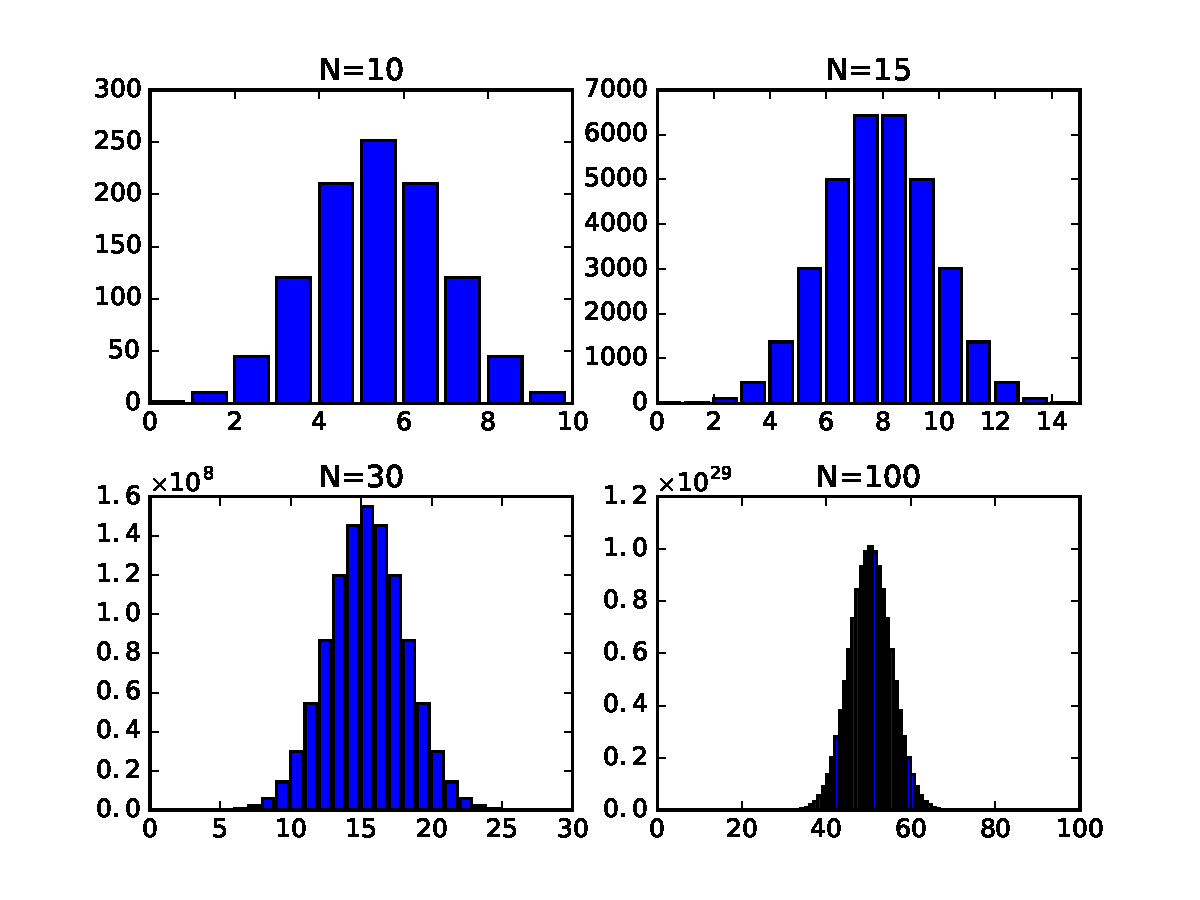
\includegraphics[width=9cm]{flip}
\caption{The number of $\Omega$ as a function of $N$ in the game of flipping coins. }
\end{figure}

\begin{figure}[h]
\centering
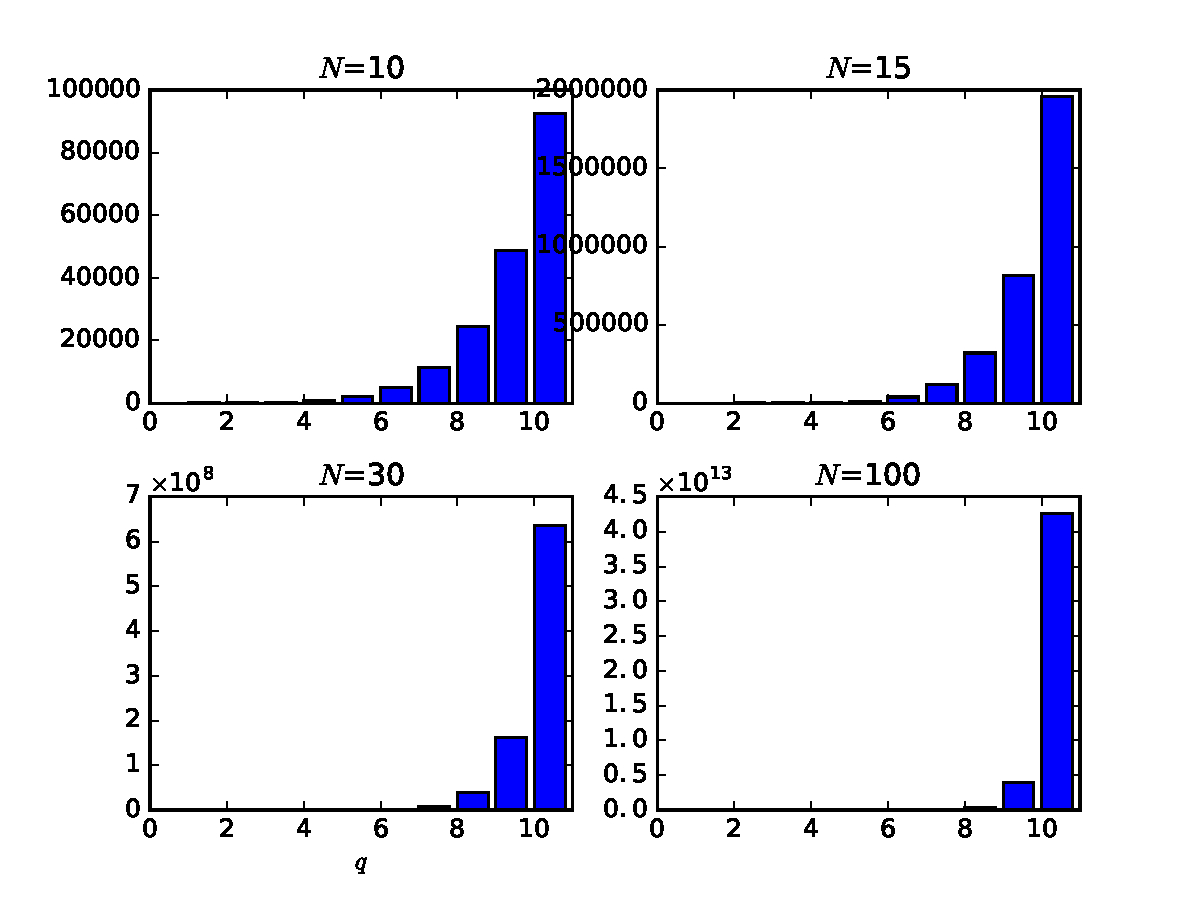
\includegraphics[width=9cm]{Einstein0}
\caption{The number of $\Omega$ as a function of $N$ in an Einstein solid. }
\end{figure}


\end{document}

